\documentclass[../main.tex]{subfiles}

\begin{document}

    \Gls{hybrid_cloud} is a very general description of an operational model.
    In order to demarcate the area of research, the environment has to be defined.

    \subsubsection{Options to delineate cloud environments}

    There are many options in terms of vendors, products and platforms providing \acrshort{iaas}, \acrshort{paas} and \acrshort{faas} that can be used to delineate a \gls{hybrid_cloud} environment.

    \acrshort{faas} is an emerging topic and very effective for dynamic scaling and cost optimization but still too immature to be considered as a major deployment style in an enterprise environment as it might not be capable of covering all needs.
    Therefore, it will not be further evaluated as part of this work.\cite{faas_status}

    \acrshort{iaas} is key to \gls{cloud_computing}, enabling on-demand self-service.
    Amazon EC2, Google Compute Engine and Azure Virtual Machines are the available services from major \gls{cloud} providers to quickly spawn virtual hardware.
    For \gls{private_cloud}, \gls{openstack} can be used to create an \acrshort{iaas} environment on-premise, but the effort it takes may not pay off.

    \acrshort{paas} is a growing market.
    Available services are, among others, \acrshort{aws} Elastic Beanstalk, Azure App Service, Google App Engine and Heroku from Salesforce.
    Despite offering almost the same capabilities, these services are prone to the lack of standardization as they are bound to a specific provider.\cite{paas_players,gartner_paas_trends}

    Two broadly applied \acrshort{paas} technologies on the market today are \gls{openshift} and \gls{cloudfoundry}.
    Both are open-source \acrshort{paas} products and can be deployed to different infrastructure providers.
    \gls{openshift} is built on top of \gls{kubernetes}.
    \gls{cloudfoundry} has its own core but started to adopt \gls{kubernetes} too.
    \gls{kubernetes} is not a traditional \acrshort{paas} solution but rather a mix of \acrshort{iaas} and \acrshort{paas}, combining the best of both worlds.
    \gls{kubernetes} has ranked as number one repository out of millions on \gls{github} based on the \glsdisp{uos}{U$\SI{}{\degree}$OS} reputation algorithm.
    With 2518 contributors and 65 440 stars as of April 2020, it is a very popular and well maintained project.
    For reference, Red Hat \gls{openshift} has ranked number seven and has 382 contributors and 7388 stars.
    \gls{cloudfoundry} does not appear on the list.\cite{github_repo_ranking,github_kubernetes,github_openshift}

    In the light of \gls{kubernetes}'s popularity and widespread use in the industry, I am using it as a basis for my research.

    \subsubsection{Kubernetes as platform}

    \acrfull{k8s} is an open-source container orchestration engine originating from Google.
    \gls{kubernetes} provides a platform to build distributed systems including services for load balancing, service discovery, health checks, configuration management, storage orchestration, deployments and rollbacks.
    Other than that, it leaves all decisions to the user.
    Unlike other products, \gls{kubernetes} does not require the use of proprietary software or a development process nor does it mandate a specific language.
    All application-level services have to be configured by the user.\cite{k8s_what_is}

    \gls{kubernetes} has become an industry standard solution for service orchestration\cite{cn_devops_with_k8s_c1}.
    It is open-source and free, which means that everyone can run their own cluster.
    Running and maintaining an own \gls{kubernetes} cluster does come at a cost though.
    Using a product as a basis for all software deployments means it becomes part of the critical infrastructure.
    As a result, a cluster has to provide high availability.
    As an alternative, fully managed \gls{kubernetes} clusters are available from all major \gls{public_cloud} providers (Table~\ref{tab:k8s_offerings}).

    \subfile{concepts-tab-k8s-hostings}

    On top of the various managed clusters, there is also a variety of custom \gls{kubernetes} distributions on the market that are tailor-made for any kind of deployment model, including not only \glsdisp{edge_cloud}{edge}- and \gls{cross_cloud} deployments but also lightweight implementations optimized for local development (Table~\ref{tab:k8s_distros}).
    In total, \gls{kubernetes} lists 57 certified distributions, 43 hostings and 18 cluster installers, all following the \gls{kubernetes} standards.\cite{k8s_conformance}

    \subfile{concepts-tab-k8s-distros}

    \gls{kubernetes} operates with manifest files that capture everything needed to run applications.
    The declarative nature of these manifests increases portability.
    Given the availability of hosting platforms, there is less risk for vendor lock-in, even when using a managed cluster of a \gls{public_cloud} provider.
    In practice, external dependencies such as storage and networking facilities may still be bound to a provider.
    Nonetheless, compared to alternative \acrshort{paas} solutions, the effort of a potential migration is viable.
    In addition, development and testing can be performed independently from the provider.

    \subsubsection{Homogeneity of the environment}

    My goal is to make the execution environment as homogeneous as possible but still profit from the flexibility of the \gls{hybrid_cloud}.
    A level of abstraction for development and operations should be achieved, which makes the \gls{hybrid_cloud} environment appear as a single unit (Fig.~\ref{fig:cloud_abstraction}).
    Virtualization lays the foundation by abstracting away the physical layer.
    Containerization builds on top of it, providing the isolation required to package it once and run it everywhere.
    \gls{kubernetes}, at last, helps to orchestrate services, without worrying too much about the physical and virtual segregation that underlies it.

    \begin{figure}[h]
        \centering
        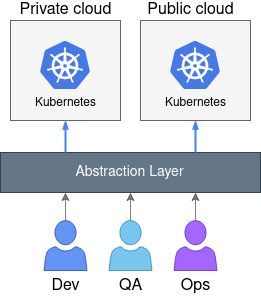
\includegraphics[width=.6\linewidth]{img/concepts_cloud_abstraction_v2.png}
        \captionsetup{justification=centering}
        \caption{
            Abstraction layer on top of the \gls{hybrid_cloud} environment for development and operations.
        }
        \label{fig:cloud_abstraction}
    \end{figure}

    Despite virtualization, containers and all the tooling on top of it, there are a few subtleties that can make a difference.
    For virtualization, different types of hypervisors might be used, which affect how operating systems communicate with the hardware and impact low-level behaviour and overall performance.
    For containers, there are multiple runtimes available.
    Containers provide isolation utilizing \gls{ns_and_cgroups}, however, the degree of isolation may vary per runtime.
    Also behaviour on kernel and system call level can be different, resulting in further variations in performance.\cite{k8s_subtl_virt,k8s_subtl_conts}

    Once \gls{kubernetes} is running with a selected container runtime, distribution and release version can still vary.
    While controlling versions of self-managed clusters is not a challenge, \gls{public_cloud} providers tend to not provide as much control.
    \acrlong{gke} has auto-upgrade capabilities and claims to make new \gls{kubernetes} versions available quickly.
    Amazon's \acrlong{eks} only supports a handful of versions and is slower in adopting new ones, taking up to three months time.
    Microsoft's \acrlong{aks} aims to adopt new versions within 30 days.
    Support for old versions is dropped within a reasonable timeframe.\cite{k8s_offering_gke,k8s_v_aks,k8s_v_eks}

    The reference environment for the instrumentation of this work has to be an easy-to-run, inexpensive \gls{hybrid_cloud} solution.
    Therefore, it will consist of a managed \gls{kubernetes} cluster from a \gls{public_cloud} provider, combined with a \gls{kubernetes} distribution optimized for local use.
    A local single-node cluster is a convenient way to conduct research and perform extensive testing without having to worry about resource usage and billing, as long as consistency, availability and partition tolerance of distributed systems is not a concern.
    The share of \gls{public_cloud} can be added in at any time, on-demand, for a proof of concept.

\end{document}

